% vim:autoindent:set textwidth=78:
\section{Getting Started}\label{label_getstarted}

This chapter gives a quick overview of running QGIS with data available on the QGIS web page.

\subsection{Installation}\label{label_installation}
\index{installation}

Building QGIS from source is documented in Appendix \ref{sec:install_windows} for windows, 
Appendix \ref{sec:install_macosx} for Mac OSX and Appendix \ref{sec:install_linux} for GNU/Linux. 
The Installation instructions are distributed with the QGIS source code and also available 
at \url{http://qgis.org}. 

Standard installer packages are available for Windows and Mac OS X. For many 
flavors of GNU/Linux binary packages are provided. Get the latest information 
on binary packages at the QGIS website at \url{http://download.qgis.org}.

\subsection{Sample Data}\label{label_sampledata}
\index{data!sample} 

If you do not have any GIS data handy, you can obtain an Alaska
dataset from the QGIS web site at \url{http://qgis.org}. The projection 
for the data is Alaska Albers Equal Area with unit meter:

\begin{verbatim}
PROJCS["NAD_1927_Albers",
    GEOGCS["GCS_North_American_1927",
	DATUM ["D_North_American_1927",
	     SPHEROID["Clarke_1866", 6378206.4,294.9786982]],
	     PRIMEM["Greenwich",0.0],
	     UNIT["Degree", 0.0174532925199433]],
    PROJECTION["Albers"],
    PARAMETER["False_Easting", 0.0],
    PARAMETER["False_Northing",0.0],
    PARAMETER["Central_Meridian",-154.0],
    PARAMETER["Standard_Parallel_1", 55.0],
    PARAMETER["Standard_Parallel_2",65.0],
    PARAMETER ["Latitude_Of_Origin",50.0],
    UNIT["Meter",1.0]]
\end{verbatim}

For use with GRASS, a sample GRASS database (e.g. Spearfish) can be obtained 
from the official GRASS GIS-website \url{http://grass.osgeo.org/download/data.php}. 
The projection of the Spearfish dataset is UTM Zone 13, Northern Hemisphere: 

\begin{verbatim}
PROJCS["UTM Zone 13, Northern Hemisphere",
    GEOGCS["clark66",
        DATUM["North_American_Datum_1927",
            SPHEROID["clark66",6378206.4,294.9786982]],
        PRIMEM["Greenwich",0],
        UNIT["degree",0.0174532925199433]],
    PROJECTION["Transverse_Mercator"],
    PARAMETER["latitude_of_origin",0],
    PARAMETER["central_meridian",-105],
    PARAMETER["scale_factor",0.9996],
    PARAMETER["false_easting",500000],
    PARAMETER["false_northing",0],
    UNIT["meter",1]]
\end{verbatim}

These data sets will be used as a basis for many of the examples and 
screenshots in this document.

\subsection{Starting QGIS}\label{label_startinqgis}

\begin{itemize}
\item \nix{assuming that QGIS is installed in the PATH, you can start QGIS by typing: \usertext{qgis}  at a command prompt or by double clicking on the QGIS
application link (or shortcut) on the desktop.} 
\item \win{start QGIS using the Start menu or desktop shortcut.}
\item \osx{double click the icon in your Applications folder.}
\end{itemize} 

\subsubsection{Command Line Options}\index{command line options}
\label{label_commandline}

QGIS supports a number of options when started from the command line. To
get a list of the options, enter \usertext{qgis ---help} on the command line.
The usage statement for QGIS is:

\small
\begin{verbatim}
qgis --help
Quantum GIS - 0.9.0 'Ganymede'
Quantum GIS (QGIS) is a viewer for spatial data sets, including
raster and vector data.
Usage: qgis [options] [FILES]
  options:
        [--snapshot filename]   emit snapshot of loaded datasets to given file
        [--lang language]       use language for interface text
        [--project projectfile] load the given QGIS project
        [--extent xmin,ymin,xmax,ymax]  set initial map extent
        [--help]                this text

  FILES:
    Files specified on the command line can include rasters,
    vectors, and QGIS project files (.qgs):
     1. Rasters - Supported formats include GeoTiff, DEM
        and others supported by GDAL
     2. Vectors - Supported formats include ESRI Shapefiles
        and others supported by OGR and PostgreSQL layers using
        the PostGIS extension
\end{verbatim}
\normalsize

\begin{Tip} \caption{\textsc{Example Using command line arguments}}
\qgistip{You can start QGIS by specifying one or more data files
on the command line. For example, assuming you are in your data directory,
you could start QGIS with two shapefiles and a raster file set to
load on startup using the following command: 
\usertext{qgis ak\_shade.tif alaska.shp majrivers.shp}
}
\end{Tip}

\minisec{Command line option \usertext{---snapshot}}
This option allows you to create a snapshot in PNG format from the current view.
This comes in handy when you have a lot of projects and want to 
generate snapshots from your data.

Currently it generates a PNG-file with 800x600 pixels. A filename can be added after
\usertext{---snapshot}.

\minisec{Command line option \usertext{---lang}}
Based on your locale QGIS, selects the correct localization. If you like to 
change your language, you can provide another language code. E.g.: 
\usertext{---lang=it}
starts QGIS in italian localization. A list of currently supported
languages with language code is provided at
\url{http://wiki.qgis.org/qgiswiki/TranslatorsCorner} 

\minisec{Command line option \usertext{---project}}
Starting QGIS with an existing project file is also possible. Just
add the command line option usertext{--project} followed by your project name
and QGIS will open with all layers loaded described in the given file.

\minisec{Command line option \usertext{---extent}}
To start with a specific map extent use this option. You need to add the bounding
box of your extent in the following order separated by a comma:
\begin{verbatim}
--extent xmin,ymin,xmax,ymax
\end{verbatim}


\subsection{QGIS GUI}\index{main window}
\label{label_qgismainwindow}

When QGIS starts, you are presented with the GUI as shown below
(the numbers 1 through 6 in blue ovals refer to the six major areas of the
interface as discussed below):

\begin{figure}[ht]
   \begin{center}
   \caption{Main window with alaska sample data (GNU/Linux with KDE)}\label{fig:startup}
   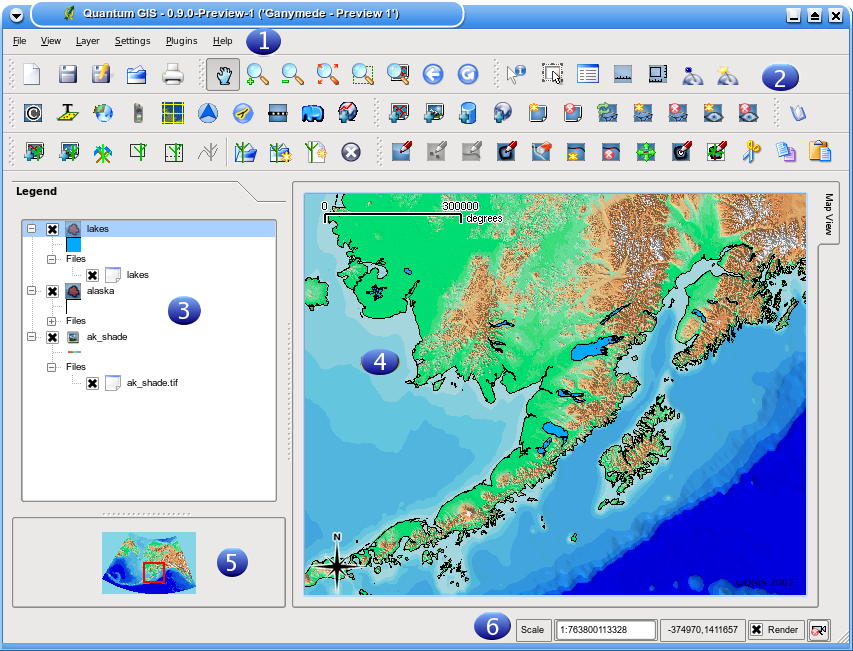
\includegraphics[clip=true, width=17cm]{startup09}
\end{center} 
\end{figure}

\textbf{Note:} Your window decorations (title bar, etc.) may appear
different depending on your operating system and window manager.

The QGIS GUI is divided into six areas:

\begin{tabbing}
1. Menu Bar \hspace{3cm}\= 4. Map View \\
2. Tool Bar \hspace{3cm}\> 5. Map Overview  \\
3. Map Legend \hspace{3cm}\> 6. Status Bar   
\end{tabbing}

These six components of the QGIS interface are described in more detail in
the following sections.

\subsubsection{Menu Bar}\label{label_menubar}
\index{menus}

The menu bar provides access to various QGIS features using a standard 
hierarchical menu. The top-level menus and a summary of some of the
functions provided are:

\begin{itemize}
\item \mainmenuopt{File}
\begin{itemize}
\item \dropmenuopt{New Project}          - see Section \ref{sec:projects}
\item \dropmenuopt{Open Project}         - see Section \ref{sec:projects}
\item \dropmenuopt{Open Recent Projects} - see Section \ref{sec:projects}
\item \dropmenuopt{Save Project}         - see Section \ref{sec:projects}
\item \dropmenuopt{Save Project As}      - see Section \ref{sec:projects}
\item \dropmenuopt{Save as Image}
\item \dropmenuopt{Export to MapServer Map}       - see Section \ref{sec:mapserver_export}
\item \dropmenuopt{Print}                         - see Section \ref{label_mapcomposer}
\item \dropmenuopt{Exit}
\end{itemize}

\item \mainmenuopt{View}
\begin{itemize}
\item \dropmenuopt{Zoom Full}
\item \dropmenuopt{Zoom To Selection}
\item \dropmenuopt{Zoom To Layer}
\item \dropmenuopt{Zoom Last}
\item \dropmenuopt{Refresh}
\item \dropmenuopt{Show Bookmarks}
\item \dropmenuopt{New Bookmark}
\item \dropmenuopt{Show most toolbars}
\item \dropmenuopt{Hide most toolbars}
\item \dropmenuopt{Toolbar Visibility} 
\end{itemize}

\item \mainmenuopt{Layer}
\begin{itemize}
\item \dropmenuopt{Add a Vector Layer}       - see Section \ref{label_workingvector}
\item \dropmenuopt{Add a Raster Layer}       - see Section \ref{label_raster}
\item \dropmenuopt{Add a PostGIS Layer}      - see Section \ref{label_postgis}
\item \dropmenuopt{Add a WMS Layer}          - see Section \ref{sec:ogc-wms}
\item \dropmenuopt{Remove Layer}
\item \dropmenuopt{New Vector Layer}          	- see Section \ref{sec:create shape}
\item \dropmenuopt{In Overview}
\item \dropmenuopt{Add All To Overview}
\item \dropmenuopt{Remove All From Overview}
\item \dropmenuopt{Hide All Layers}
\item \dropmenuopt{Show All Layers}
\end{itemize}

\item \mainmenuopt{Settings}
\begin{itemize}
\item \dropmenuopt{Project Properties}  - see Section \ref{sec:projects}
\item \dropmenuopt{Custom Projection}   - see Section \ref{sec:customprojections}
\item \dropmenuopt{Options}             - see Section \ref{subsec:gui_options}
\end{itemize}

\item \mainmenuopt{Plugins} - (Futher menu items are added by plugins as they are loaded.)
\begin{itemize}
\item \dropmenuopt{Plugin Manager}          	   - see Section \ref{sec:managing_plugins}
\end{itemize}          	

\item \mainmenuopt{Help}
\begin{itemize}
\item \dropmenuopt{Help Contents}
\item \dropmenuopt{QGIS Homepage}
\item \dropmenuopt{Check QGIS Version}
\item \dropmenuopt{About}
\end{itemize}

\end{itemize}

%See Appendix \ref{app_menu} for complete descriptions of the menu items.

\subsubsection{Toolbars}\label{label_toolbars}
\index{toolbars}

The toolbars provide access to most of the same functions as the menus,
plus additional tools for interacting with the map. Each toolbar item has
popup help available. Hold your mouse over the item and a short description of
the tool's purpose will be displayed. 

Every menubar can be moved around according to your needs. Additionally every
menubar can be switched off using your right mouse button context menu holding
the mouse over the toolbars.

\begin{Tip}
\caption{\textsc{Reappearing toolbars}} \index{layout!toolbars}
\qgistip{If you have accidentally hidden all your toolbars, you can get them back by
choosing menu option \mainmenuopt{View} > \dropmenuopt{Show most toolbars}.}
\end{Tip}

\subsubsection{Map Legend}\label{label_legend}
\index{legend}

% TODO The new legend features need to be described here briefly.
% Marco, would you make a start what is new in the legend?!
The map legend area is used to set the visibility and z-ordering of layers.
Z-ordering means that layers listed nearer the top of the legend are drawn
over layers listed lower down in the legend. The checkbox in each legend
entry can be used to show or hide the layer.\index{layer!visibility}

Layers can be grouped in the legend window by adding a layer group and dragging layers 
into the group. To do so, go with the mouse to the legend window, right click, choose \dropmenuopt{Add group}. 
A new folder appears. Now drag the layers to the folder symbol. It is then possible to toggle the 
visibility of all the layers in the group with one click. To bring layers out of a group, go with 
the mouse to the layer symbol, right click, choose \dropmenuopt{Make to toplevel item}. To give the folder a 
new name, choose \dropmenuopt{Rename} in the right click menu of the group.

The content of the right mouse button context menu depends on if the loaded legend item you hold your 
mouse over is a raster or a vector layer. For GRASS vector layers the \dropmenuopt{toggle editing} is not 
available. See section \ref{grass_digitising} for infos on editing GRASS vector layers. 

\begin{itemize}

\item \textbf{Right mouse button menu for raster layers}
\begin{itemize}
\item \dropmenuopt{Zoom to layer extent}
\item \dropmenuopt{Zoom to best scale (100\%)}
\item \dropmenuopt{Show in overview}
\item \dropmenuopt{Remove}
\item \dropmenuopt{Properties}
\item \dropmenuopt{Rename}
\item \dropmenuopt{Add Group}
\item \dropmenuopt{Expand all}
\item \dropmenuopt{Collapse all}
\item \dropmenuopt{Show file groups}
\end{itemize}

\item \textbf{Right mouse button menu for vector layers}
\begin{itemize}
\item \dropmenuopt{Zoom to layer extent}
\item \dropmenuopt{Show in overview}
\item \dropmenuopt{Remove}
\item \dropmenuopt{Open attribute table}
\item \dropmenuopt{Toggle editing (not available for GRASS layers)}
\item \dropmenuopt{Save as shapefile}
\item \dropmenuopt{Save selection as shapefile}
\item \dropmenuopt{Properties}
\item \dropmenuopt{Rename}
\item \dropmenuopt{Add Group}
\item \dropmenuopt{Expand all}
\item \dropmenuopt{Collapse all}
\item \dropmenuopt{Show file groups}
\end{itemize}

\item \textbf{Right mouse button menu for layer groups} 
\begin{itemize}
\item \dropmenuopt{Remove}
\item \dropmenuopt{Rename}
\item \dropmenuopt{Add Group}
\item \dropmenuopt{Expand all}
\item \dropmenuopt{Collapse all}
\item \dropmenuopt{Show file groups}
\end{itemize}

\end{itemize}

If several vector data sources have the same vector type and the same attributes, their 
symbolisations may be grouped. This means that if the symbolisation of one data source is 
changed, the others automatically have the new symbolisation as well. To group symbologies, open 
the right click menu in the legend window and choose \menuopt{Show file groups}. The file groups of the 
layers appear. It is now possible to drag a file from one file group into another one. If this is done, 
the symbologies are grouped. Note that QGIS only permits the drag if the two layers are able to share 
symbology (same vector type and same attributes).  

%% isn't included in Titan anymore, except for an "toggle overview"
%Each legend entry can show the following mini icons:
%
%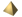
\includegraphics[width=0.7cm]{pyramid} This is a raster
%that has pyramids built for it to improve rendering efficiency (see
%Section \ref{raster_pyramids}).\\
%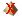
\includegraphics[width=0.7cm]{no_pyramid} This is a
%raster that has no pyramid layers (see Section \ref{raster_pyramids}).\\
%
\includegraphics[width=0.7cm]{inoverview} This layer is
%shown in the overview map area as well as in the main map window.\\
%
\includegraphics[width=0.7cm]{editable} This is a vector
%layer that is currently enabled for editing.\\

\subsubsection{Map View}\label{label_mapview}
\index{map!view}

This is the 'business end' of QGIS - maps are displayed in this area! The
map displayed in this window will depend on the vector and raster layers you
have chosen to load (see sections that follow for more information on how to
load layers). The map view can be panned (shifting the focus of the map display
to another region) and zoomed in and out. Various other operations can be
performed on the map as described in the toolbar description above.  The map
view and the legend are tightly bound to each other - the maps in view reflect
changes you make in the legend area.  

\begin{Tip}\caption{\textsc{Zooming the Map with the Mouse
Wheel}}\index{zoom!mouse wheel}
\qgistip{You can use the mouse wheel to zoom in and out on the map. Place
the mouse cursor inside the map area and roll it forward (away from you) to
zoom in and backwards (towards you) to zoom out. The mouse cursor is the 
center where the zoom occurs. You can customize the behavior of the mouse
wheel zoom using the \tab{Map tools} tab under the \mainmenuopt{Settings} >\dropmenuopt{Options} menu.  }
\end{Tip}

\subsubsection{Map Overview}\label{label_mapoverview}
\index{map!overview}

The map overview area provides a full extent view of layers added to it.
Within the view is a rectangle showing the current map extent. This allows
you to quickly determine which area of the map you are currently viewing. Note
that labels are not rendered to the map overview even if the layers in the
map overview have been set up for labeling. 
You can add a single layer to the
overview by right-clicking on it in the legend and choosing \dropmenuopt{Show in overview}. You can also add or remove all layers to the overview using the
Overview tools on the toolbar.

You can also grab the red rectangle showing your current extent and pan around; the
map view will update accordingly.

\subsubsection{Status Bar}\label{label_statusbar}

The status bar shows you your current position in map coordinates (e.g.
meters or decimal degrees) as the mouse pointer is moved across the map view.
The status bar also shows the view extents of the map view as you pan and
zoom in and out. A progress bar in the status bar shows progress of rendering
as each layer is drawn to the map view. In some cases, such as the gathering
of statistics in raster layers, the progress bar will be used to show the
status of lengthy operations. On the right side of the status bar is a small
checkbox which can be used to temporarily prevent layers being rendered to the
map view (see Section \ref{subsec:redraw_events} below). At the far right of
the status bar is a projector icon. Clicking on this opens the projection
properties for the current project.

\subsection{Rendering}\label{subsec:redraw_events}\index{rendering}

By default, QGIS renders all visible layers whenever the map canvas must be
refreshed. The events that trigger a refresh of the map canvas include:

\begin{itemize}
\item Adding a layer
\item Panning or zooming
\item Resizing the QGIS window
\item Changing the visibility of a layer or layers
\end{itemize}

QGIS allows you to control the rendering process in a number of ways.

\subsubsection{Scale Dependent Rendering}\index{rendering!scale dependent}
\label{label_scaledepend}

Scale dependent rendering allows you to specify the minimum and maximum
scales at which a layer will be visible.  To set scale dependency rendering,
open the \dialog{Properties} dialog by double-clicking on the layer in the legend. On
the \tab{General} tab, set the minimum and maximum scale values and then
click on the \checkbox{Use scale dependent rendering} checkbox.

You can determine the scale values by first zooming to the level you want
to use and noting the scale value in the QGIS status bar.\index{scale}

\subsubsection{Controlling Map Rendering}\label{label_controlmap}

Map rendering can be controlled in the following ways:

\minisec{Suspending Rendering}\index{rendering!suspending}
\label{label_suspendrender}

To suspend rendering, click the \checkbox{Render} checkbox in the lower right
corner of the statusbar. When the \checkbox{Render} box is not checked, QGIS
does not redraw the canvas in response to any of the events described in
Section \ref{subsec:redraw_events}. Examples of when you might want to suspend
rendering include:

\begin{itemize}
\item Add many layers and symbolize them prior to drawing
\item Add one or more large layers and set scale dependency before drawing
\item Add one or more large layers and zoom to a specific view before
drawing
\item Any combination of the above
\end{itemize}

Checking the \checkbox{Render} box enables rendering and causes and immediate
refresh of the map canvas.

\minisec{Setting Layer Add Option}\label{label_settinglayer}
\index{rendering!options}\index{layers!initial visibility}

You can set an option to always load new layers without drawing them. This
means the layer will be added to the map, but its visibility checkbox in the
legend will be unchecked by default. To set this option, choose
menu option \mainmenuopt{Settings} > \dropmenuopt{Options} and click on the
\tab{Rendering} tab. Uncheck the \checkbox{By default new layers added to the map 
should be
displayed} checkbox. Any layer added to the map will be off (invisible) by
default.

%\minisec{Stopping Rendering}\index{rendering!halting}
%\label{label_stoprender}
%
%To stop the map drawing, press the ESC key. This will halt the refresh of
%the map canvas and leave the map partially drawn. It may take a bit of time
%between pressing ESC and the time the map drawing is halted.
%
%\textbf{NOTE}: It is currently not possible to stop rendering - this was disabled 
%in qt4 port because of User Interface (UI) problems and crashes.

\minisec{Updating the Map Display During Rendering}
\label{label_updatemap}\index{rendering!update during drawing}

You can set an option to update the map display as features are drawn. By
default, QGIS does not display any features for a layer until the entire
layer has been rendered. To update the display as features are read from the
datastore, choose menu option \mainmenuopt{Settings} > \dropmenuopt{Options}
click on the \tab{Rendering} tab. Set the feature count to an
appropriate value to update the display during rendering. Setting a value of 0
disables update during drawing (this is the default). Setting a value too low
will result in poor performance as the map canvas is continually updated
during the reading of the features. A suggested value to start with is 500. 

\subsection{Measuring}\label{sec:measure}\index{measure}

Measuring works within projected coordinate systems only (e.g., UTM). If 
the loaded map is defined with a geographic coordinate system
(latitude/longitude), the results from line or area measurements will be 
incorrect. To fix this you need to set an appropriate map coordinate system.

\subsubsection{Measure length}\index{measure:line length}

\includegraphics[width=0.7cm]{measureline} QGIS is also able to measure real distances between given 
points according to a defined ellipsoid. Therefore choose menu option \mainmenuopt{Settings} > \dropmenuopt{Options}, 
click on the \tab{Map tools} tab and choose the appropriate ellipsoid. The tool then allows you to 
click points on the map. Each segment-length shows up in the measure-window and additionaly the total 
length is printed. To stop measuring click your right mouse button. 

\subsubsection{Measure areas}\index{measure:areas}

\includegraphics[width=0.7cm]{measurearea} Also areas can be measured. The window only shows the
accumulated area-size in the measure window (see figure \ref{fig:measure}).

% measure-tools side by side
\begin{figure}[h]
\caption{Measure tools in action} \label{fig:measure}
\centering
   \subfigure[Measure lines] {\label{subfig:measure_line}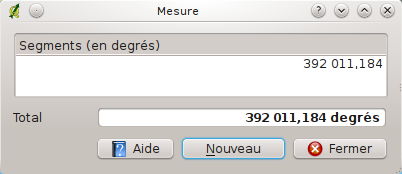
\includegraphics[clip=true, width=0.4\textwidth]{measure_line}}\goodgap
   \subfigure[Measure areas]{\label{subfig:measure_area}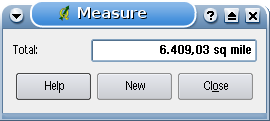
\includegraphics[clip=true, width=0.4\textwidth]{measure_area}}
\end{figure}

\subsection{Projects}\label{sec:projects}\index{projects}

The state of your QGIS session is considered a Project.  QGIS
works on one project at a time.  Settings are either considered
as being per-project, or as a default for new projects (see
Section \ref{subsec:gui_options}).

QGIS can save the state of your workspace into a project file using
the menu option \mainmenuopt{File} > \dropmenuopt{Save Project}.

Loading saved projects is a similar process.

The kinds of information saved in a project file include:

\begin{itemize}
\item Layers added
\item Layer properties, including symbolization
\item Projection for the map view
\item Last viewed extent
\end{itemize}

The project file is saved in XML format, so it is possible to edit
the file outside QGIS if you know what you are doing.  

The file format was updated several times compared to earlier QGIS versions. Project files 
from older QGIS versions may not work properly anymore.

\subsection{GUI Options}
\label{subsec:gui_options}

\includegraphics[width=0.7cm,clip=true]{mActionOptions} Some basic options for QGIS
can be selected using the \dialog{Options} dialog. Select the 
menu option \mainmenuopt{Settings} >
 \dropmenuopttwo{mActionOptions}{Options} or press \keystroke{Alt-O}. The tabs where you can 
optmize your options are:

\minisec{General Tab}

\begin{itemize}
\item Ask to save project changes when required
\end{itemize}

\minisec{Appearance Tab}

\begin{itemize}
\item Hide or show splash screen at startup
\item Change the icon theme 
\item Change Selection and backgroud Color
\item Make layer names appear with Capitals
\end{itemize}

\minisec{Rendering Tab}

\begin{itemize}
\item Update features during drawing or not until all features have been read.
\item Set new layer visible or unvisible when loaded 
\item Make lines appear less jagged at the expense of some drawing performance
\item Fix problems with incorrectly filled polygons
\item Continously redraw when dragging the legend/map divider 
\end{itemize}

\minisec{Map tools Tab}

\begin{itemize}
\item Define Search Radius as a percentage of the map width
\item Define Ellipsoid for distance calculations
\item Set Rubberband Color for Measure Tool
\item Define Mouse wheel action (Zoom, Zoom and recenter, Nothing)
\item Set Zoom factor for wheel mouse
\end{itemize}

\minisec{Projection Tab}

\begin{itemize}
\item Define what to do, when a layer is loaded without projection information
\begin{itemize}
\item Prompt for projection
\item Project wide default projection will be used
\item Global default projection displayed below will be used
\end{itemize}
\end{itemize}

\minisec{Locale Tab}

\begin{itemize}
\item Overwrite system locale and use defined locale instead
\item Information about active system locale
\end{itemize}

\minisec{Help Browser Tab}

\begin{itemize}
\item Define Browser to display help documents
\end{itemize}


You can modify the options according to your needs. Some of the changes may 
require a restart of QGIS before they will be effective.

\begin{itemize}
\item \nix{everything is saved in:}
\begin{verbatim}
$HOME/.config/QuantumGIS/qgis.conf
\end{verbatim}
This is a normal text file consisting of blocks, where QGIS saves its current
display options, PostGIS and WMS connections, and other settings.

\item \win{settings are stored in the registry under:}
\begin{verbatim}
\\HKEY_CURRENT_USER\Software\QuantumGIS\qgis
\end{verbatim}

\item \osx{you can find your settings in:}
\begin{verbatim}
$HOME/Library/Preferences/org.qgis.qgis.plist
\end{verbatim}
\end{itemize}


\subsection{Spatial Bookmarks}\label{sec:bookmarks}
\index{bookmarks}
\index{spatial bookmarks|\see{bookmarks}}

Spatial Bookmarks allow you to ``bookmark'' a geographic location and return to it later.

\subsubsection{Creating a Bookmark}
To create a bookmark:
\begin{enumerate}
\item Zoom or pan to the area of interest.
\item Select the menu option \mainmenuopt{View} > \dropmenuopt{New Bookmark} or press \keystroke{Ctrl-B}.
\item Enter a descriptive name for the bookmark (up to 255 characters).
\item Click \button{OK} to add the bookmark or \button{Cancel} to exit without adding the bookmark.
\end{enumerate}

Note that you can have multiple bookmarks with the same name.

\subsubsection{Working with Bookmarks}
To use or manage bookmarks, select the menu 
option \mainmenuopt{View} > \dropmenuopt{Show Bookmarks}.
The \dialog{Geospatial Bookmarks} dialog allows you to zoom to or delete a bookmark.
You can not edit the bookmark name or coordinates.

\subsubsection{Zooming to a Bookmark}
From the \dialog{Geospatial Bookmarks} dialog, select the desired bookmark by clicking on it, 
then click \button{Zoom To}.
You can also zoom to a bookmark by double-clicking on it.

\subsubsection{Deleting a Bookmark}
To delete a bookmark from the \dialog{Geospatial Bookmarks} dialog, click on it then click
 \button{Delete}.
Confirm your choice by clicking \button{Yes} or cancel the delete by clicking \button{No}.
